\documentclass[]{article}
\usepackage[english,ngerman]{babel}
\usepackage[utf8]{inputenc}
\usepackage{graphicx}
\linespread{1.2}

%opening
\title{Matrix-Multiplikatin}
\author{Mark Geiger \and Rico Fritzsche}

\begin{document}

\maketitle

\begin{abstract}
Im Kurs Parallele Programmierung soll der Geschwindigkeitsunterschied verschiedener Umsetzungen der Matrixmultiplikation demonstriert werden. Dazu wurde ein Testprogramm erstellt, welches unterschiedliche Konzepte umsetzt und zeitlich bewertet. Zur Auswertung wurde ein Python-Skript erstellt, welches die Zeit als Funktion der Matrixgröße darstellt.
\end{abstract}

\section*{Umsetzung}
In der Übung wurden die Multiplikation für quatratische Matrizen umgesetzt. Dazu sind wir in vier Schritten vorgegangen, um eine effizientere Geschwindigkeit der Operationen erzielen zu können. Jeder Schritt setzt eine eigene Implementierung der Multiplikation um. Begonnen haben wir mit der naiven Multiplikation. Diese durchläuft die Spalten der ersten Matrix und die Zeilen der zweiten Matrix, multipliziert diese und summiert die Ergebnisse. Aufgrund des zu kleinen Stacks, müssen die Matrizen mit dem C-Befehl \textit{malloc()} angelegt werden, welcher Speicher auf dem Heap reserviert. Im zweiten Schritt haben wir den Blocke-Ansatz umgesetzt. Mit Recherche im Internet haben wir herausgefunden, dass wir zunächst mittels Schleifen festlegen müssen, in welchen Schritten das Programm die Blöcke der Matrizen durchlaufen soll. Innerhalb dieser Schleifen kann analog zu der naiven Implementierung vorgegangen werden. Dieser Ansatz zeigt im Vergleich zur naiven Implementierung einen deutlichen Geschwindigkeitsvorteil. Im dritten Schritt wurde die Bibliothek BLAS zur Berechnung der Matrixmultiplikation genutzt. Diese stellt nach der Einbindung mittels \textit{\#include cblas.h} die Funktion \textit{cblas\_dgemm()} bereit. Ihr werden unter anderem die Eingangsmatrizen übergeben, das Ergebnis wird als Pointer zurückgegeben. Auch hier konnten wir im Vergleich zu den vorherigen Ergebnissen eine Geschwindkeitszunahme der Matrixmultiplikation erkennen. Für die letzte Anforderung haben wir den Blocked-Ansatz mittels SIMD (Single iInstruction, Multiple Data) optimiert. Dabei werden zur Berechnung die SSE (Streaming SIMD Extensions)-Einheiten des Prozessors verwendet. Diese wurden für Gleitkommazahl entwickelt und haben das Ziel auf der Instruktionsebene Programme mittels Parallelisierung zu beschleunigen. Für die Umsetzung mussten wir auf Quellen\footnote{http://download.intel.com/design/PentiumIII/sml/24504501.pdf} im Internet zurückgreifen. 

\section*{Ergebnisse}
Damit die Ergebnisse verglichen werden können, wird die Funktion \textit{get\_time()} und \textit{timespec\_diff()} verwendet, welches über \textit{\#include \glqq timing.h\grqq} zur Verfügung stehen. Durch den Aufruf vor und nach der implementierten Matrixmultiplikation wird mittels Differenz die benötigte Zeit ermittelt. Da wir die Implementierung der BLAS-Funktionen nicht kennen, kann keine korrekte Aussage über die verwendeten Gleitkommaoperationen getroffen werden. Aus diesem Grund ist ein direkter Vergleich von MFLOPS der Ansätze nicht möglich. \\
Zur Auswertung werden die vier Testimplementationen mit verschiedenen Matrixgrößen wiederholt. Die Größe der Matrizen orientiert sich an der Zweier-Potenzreihe im Bereich von 16 bis 2048. Anschließend werden die Größen sowie die zur Berechnung benötigte Zeit für jeden Ansatz der Matrixmultiplikation in eine Textdatei gespeichert. Ein Python-Skript liest diese Datei ein und plottet die Ergbnisse in einem Liniendiagramm \ref{pic:ergebnis}. Es ist zu erkennen, dass die Umsetzung der BLAS-Bibliothek eine sehr effiziente Lösung bereitstellt. Auch die SIMD-Implementierung des Blocked-Ansatz stellt eine effiziente Implementierung dar, ist jedoch marginal langsamer als die BLAS-Implementierung. Damit kann gezeigt werden, dass durch Parallelisierung eine deutliche Leistungssteigerung durch eine erhöhte Geschwindigkeit zu erreichen ist.

\section*{Ausführung}
\textit{make}\\
\textit{make run}\\
\textit{make plot}

\begin{figure}[h]
	\centering
	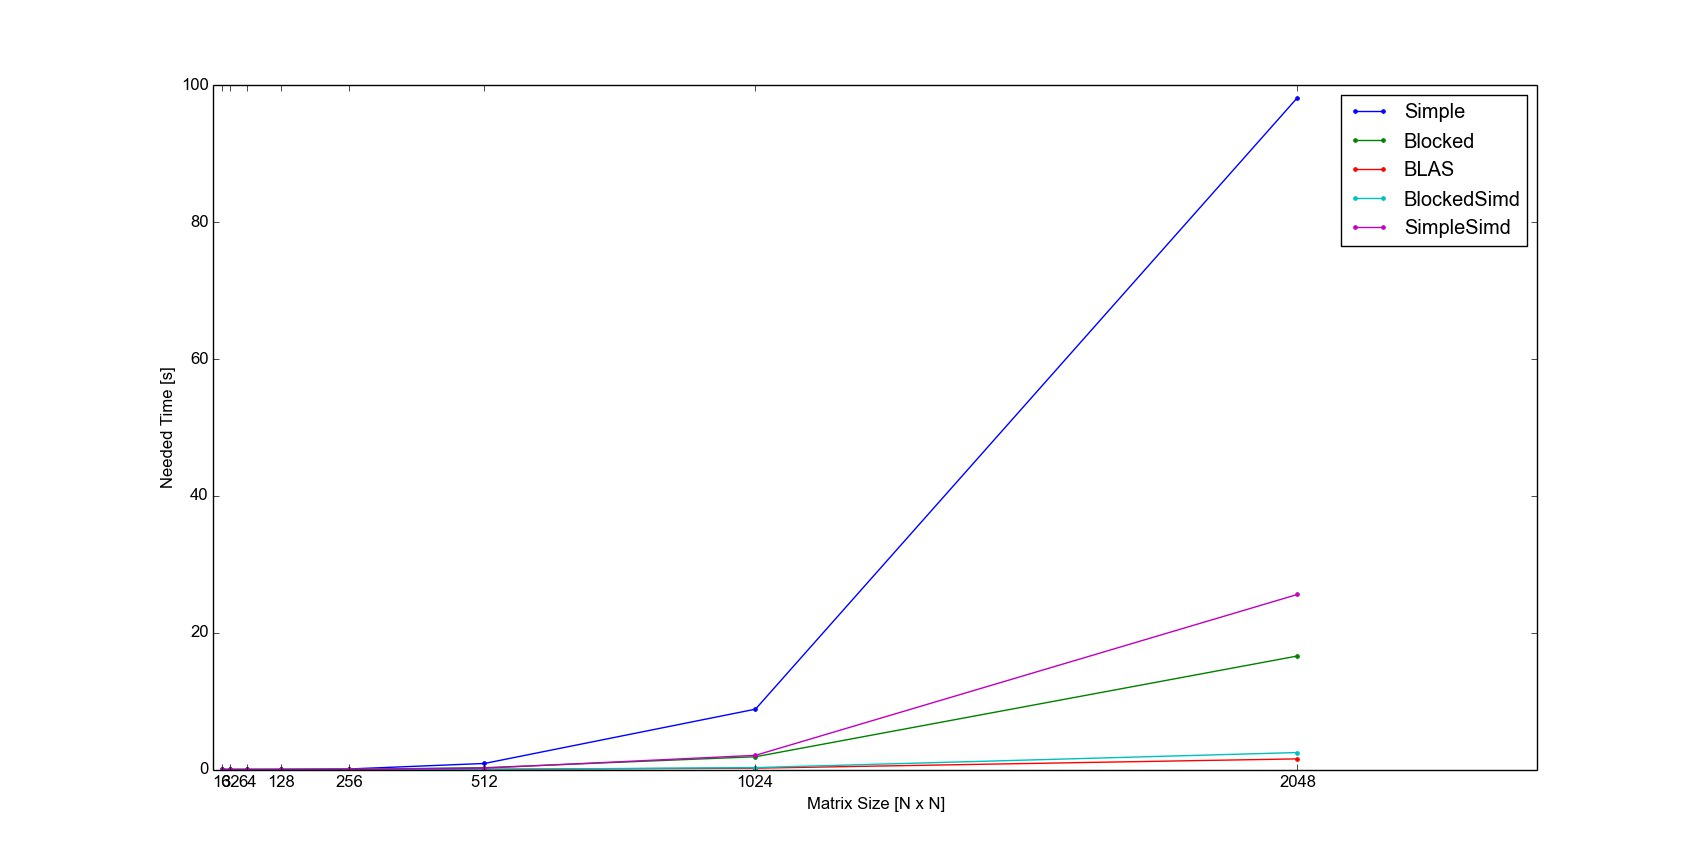
\includegraphics[width=1\linewidth]{ergebnis.jpg}
	\caption{Ergebnis der Testimplementation, dargestellt mittels Python-Scripts}
	\label{pic:ergebnis}
\end{figure}
\end{document}
